\chapter{Classical synchronization problems}

In this chapter we examine the classical problems that appear
in nearly every operating systems textbook.  They
are usually presented in terms of real-world problems, so
that the statement of the problem is clear and so that students
can bring their intuition to bear.

For the most part, though, these problems do not happen in the
real world, or if they do, the real-world solutions are not much
like the kind of synchronization code we are working with.

The reason we are interested in these problems
is that they are analogous to common problems that operating
systems (and some applications) need to solve.  For each classical
problem I will present the classical formulation, and also explain
the analogy to the corresponding OS problem.


\section{Producer-consumer problem}

In multithreaded programs there is often a division of labor between
threads.  In one common pattern, some threads are producers and some
are consumers.  Producers create items of some kind and add them to a
data structure; consumers remove the items and process them.

Event-driven programs are a good example.  An ``event'' is something
that happens that requires the program to respond: the user presses a
key or moves the mouse, a block of data arrives from the disk, a
packet arrives from the network, a pending operation completes.

Whenever an event occurs, a producer thread creates an event
object and adds it to the event buffer.  Concurrently, consumer
threads take events out of the buffer and process them.
In this case, the consumers are called ``event handlers.''

There are several synchronization constraints that we need to
enforce to make this system work correctly:

\begin{itemize}

\item While an item is being added to or removed from the buffer,
the buffer is in an inconsistent state.  Therefore, threads must
have exclusive access to the buffer.

\item If a consumer thread arrives while the buffer is empty, it
blocks until a producer adds a new item.

\end{itemize}

Assume that producers perform the following operations over and
over:

\begin{lstlisting}[title={Basic producer code}]{}
event = waitForEvent()
buffer.add(event)
\end{lstlisting}

Also, assume that consumers perform the following operations:

\begin{lstlisting}[title={Basic consumer code}]{}
event = buffer.get()
event.process()
\end{lstlisting}

As specified above, access to the buffer has to be exclusive,
but {\tt waitForEvent} and {\tt event.process}
can run concurrently.

Puzzle: Add synchronization statements to the producer and
consumer code to enforce the synchronization constraints.

\clearemptydoublepage
\subsection{Producer-consumer hint}

Here are the variables you might want to use:

\begin{lstlisting}[title={Producer-consumer initialization}]{}
mutex = Semaphore(1)
items = Semaphore(0)
local event
\end{lstlisting}

Not surprisingly, {\tt mutex} provides exclusive access to
the buffer.  When {\tt items} is positive, it indicates the
number of items in the buffer.  When it is negative, it
indicates the number of consumer threads in queue.

{\tt event} is a {\bf local variable}, which in this context means
that each thread has its own version.
So far we have been assuming that all threads have access
to all variables, but we will sometimes find it useful to
attach a variable to each thread.

There are a number of ways this can be implemented in different
environments:

\begin{itemize}

\item If each thread has its own run-time stack, then any variables
allocated on the stack are thread-specific.

\item If threads are represented as objects, we can add an attribute
to each thread object.

\item If threads have unique IDs, we can use the IDs as an index
into an array or hash table, and store per-thread data there.

\end{itemize}

In most programs, most variables are local unless declared otherwise,
but in this book most variables are shared, so we will assume that
that variables are shared unless they are explicitly declared {\tt
local}.



\clearemptydoublepage
\subsection{Producer-consumer solution}

Here is the producer code from my solution.

\begin{lstlisting}[title={Producer solution}]{}
event = waitForEvent()
mutex.wait()
    buffer.add(event)
    items.signal()
mutex.signal()
\end{lstlisting}

The producer doesn't have to get exclusive access to the buffer
until it gets an event.  Several threads can run {\tt waitForEvent}
concurrently.

The {\tt items} semaphore keeps track of the
number of items in the buffer.  Each time the producer adds an
item, it signals {\tt items}, incrementing it by one.

The consumer code is similar.

\begin{lstlisting}[title={Consumer solution}]{}
items.wait()
mutex.wait()
    event = buffer.get()
mutex.signal()
event.process()
\end{lstlisting}

Again, the buffer operation is protected by a mutex,
but before the consumer gets to it, it has to decrement
{\tt items}.  If {\tt items} is zero or negative, the
consumer blocks until a producer signals.

Although this solution is correct, there is an opportunity
to make one small improvement to its performance.  Imagine
that there is at least one consumer in queue when a producer
signals {\tt items}.  If the scheduler allows the consumer
to run, what happens next?  It immediately blocks on the
mutex that is (still) held by the producer.

Blocking and waking up are moderately expensive operations;
performing them unnecessarily can impair the performance of
a program.  So it would probably be better to rearrange the
producer like this:

\begin{lstlisting}[title={Improved producer solution}]{}
event = waitForEvent()
mutex.wait()
    buffer.add(event)
mutex.signal()
items.signal()
\end{lstlisting}

Now we don't bother unblocking a consumer until we know it can proceed
(except in the rare case that another producer beats it to the mutex).

There's one other thing about this solution that might bother
a stickler.  In the hint section I claimed that the {\tt items}
semaphore keeps track of the number of items in queue.  But looking
at the consumer code, we see the possibility that several consumers
could decrement {\tt items} before any of them gets the mutex
and removes an item from the buffer.  At least for a little while,
{\tt items} would be inaccurate.

We might try to address that by checking the buffer inside the
mutex:

\begin{lstlisting}[title={Broken consumer solution}]{}
mutex.wait()
    items.wait()
    event = buffer.get()
mutex.signal()
event.process()
\end{lstlisting}

This is a bad idea.

Puzzle: why?


\clearemptydoublepage
\subsection{Deadlock \#4}

If the consumer is running this code

\begin{lstlisting}[title={Broken consumer solution}]{}
mutex.wait()
    items.wait()
    event = buffer.get()
mutex.signal()

event.process()
\end{lstlisting}
%
it can cause a deadlock.  Imagine that the buffer is empty.
A consumer arrives, gets the mutex, and then blocks on
{\tt items}.  When the producer arrives, it blocks on
{\tt mutex} and the system comes to a grinding halt.

This is a common error in synchronization code: any time
you wait for a semaphore while holding a mutex, there is
a danger of deadlock.  When you are checking a solution to
a synchronization problem, you should check for this kind
of deadlock.


\subsection{Producer-consumer with a finite buffer}

In the example I described above, event-handling threads,
the shared buffer is usually infinite (more accurately, it is
bounded by system resources like physical memory and swap
space).

In the kernel of the operating system, though, there are
limits on available space.  Buffers for things like disk
requests and network packets are usually fixed size.  In
situations like these, we have an additional synchronization
constraint:

\begin{itemize}

\item If a producer arrives when the buffer is full, it
blocks until a consumer removes an item.

\end{itemize}

Assume that we know the size of the buffer.  Call it
{\tt bufferSize}.  Since we have a semaphore that is keeping
track of the number of items, it is tempting to write something
like 

\begin{lstlisting}[title={Broken finite buffer solution}]{}
if items >= bufferSize:
    block()
\end{lstlisting}

But we can't.  Remember that we can't check the current
value of a semaphore; the only operations are {\tt wait}
and {\tt signal}.

Puzzle: write producer-consumer code that handles the finite-buffer
constraint.

\clearemptydoublepage
\subsection{Finite buffer producer-consumer hint}

Add a second semaphore to keep track of the number of
available spaces in the buffer.

\begin{lstlisting}[title={Finite-buffer producer-consumer initialization}]{}
mutex = Semaphore(1)
items = Semaphore(0)
spaces = Semaphore(buffer.size())
\end{lstlisting}

When a consumer removes an item it should signal {\tt spaces}.
When a producer arrives it should decrement {\tt spaces}, at
which point it might block until the next consumer signals.


\clearemptydoublepage
\subsection{Finite buffer producer-consumer solution}

Here is a solution.

\begin{lstlisting}[title={Finite buffer consumer solution}]{}
items.wait()
mutex.wait()
    event = buffer.get()
mutex.signal()
spaces.signal()

event.process()
\end{lstlisting}

The producer code is symmetric, in a way:

\begin{lstlisting}[title={Finite buffer producer solution}]{}
event = waitForEvent()

spaces.wait()
mutex.wait()
    buffer.add(event)
mutex.signal()
items.signal()
\end{lstlisting}

In order to avoid deadlock, producers and consumers check
availability before getting the mutex.  For best performance,
they release the mutex before signaling.


\section{Readers-writers problem} 

The next classical problem, called the Reader-Writer Problem, pertains
to any situation where a data structure, database, or file system is
read and modified by concurrent threads.  While the data structure is
being written or modified it is often necessary to bar other threads
from reading, in order to prevent a reader from interrupting a
modification in progress and reading inconsistent or invalid data.

As in the producer-consumer problem, the solution is asymmetric.
Readers and writers execute different code before entering the
critical section.  The synchronization constraints are:

\begin{enumerate}

\item Any number of readers can be in the critical section
simultaneously.

\item Writers must have exclusive access to the critical section.

\end{enumerate}

In other words, a writer cannot enter the critical section while
any other thread (reader or writer) is there, and while the writer
is there, no other thread may enter.

The exclusion pattern here might be called {\bf categorical
mutual exclusion}.  A thread in the critical section
does not necessarily exclude other threads, but the presence
of one category in the critical section excludes other
categories.

Puzzle: Use semaphores to enforce these constraints, while allowing
readers and writers to access the data structure, and avoiding
the possibility of deadlock.


\clearemptydoublepage
\subsection{Readers-writers hint}

Here is a set of variables that is sufficient to solve the
problem.

\begin{lstlisting}[title={Readers-writers initialization}]{}
int readers = 0
mutex = Semaphore(1)
roomEmpty = Semaphore(1)
\end{lstlisting}

The counter {\tt readers} keeps track of how many readers
are in the room.  {\tt mutex} protects the shared counter.

{\tt roomEmpty} is 1 if there are no threads (readers or writers) in
the critical section, and 0 otherwise.  This demonstrates the naming
convention I use for semaphores that indicate a condition.  In
this convention, ``wait'' usually means ``wait for the condition to
be true'' and ``signal'' means ``signal that the condition is true''.


\clearemptydoublepage
\subsection {Readers-writers solution}

The code for writers is simple.  If the critical section
is empty, a writer may enter, but entering has the effect
of excluding all other threads:

\begin{lstlisting}[title={Writers solution}]{}
roomEmpty.wait()
    critical section for writers
roomEmpty.signal()
\end{lstlisting}

When the writer exits, can it be sure that the room is
now empty?  Yes, because it knows that no other thread can
have entered while it was there.

The code for readers is similar to the barrier code we
saw in the previous section.  We keep track of the number
of readers in the room so that we can give a special assignment
to the first to arrive and the last to leave.

The first reader that arrives has to wait for {\tt roomEmpty}.
If the room is empty, then the reader proceeds and, at the
same time, bars writers.  Subsequent readers can still enter
because none of them will try to wait on {\tt roomEmpty}.

If a reader arrives while there is a writer in the room,
it waits on {\tt roomEmpty}.  Since it holds the mutex, any
subsequent readers queue on {\tt mutex}.

\begin{lstlisting}[title={Readers solution}]{}
mutex.wait()
    readers += 1
    if readers == 1:
        roomEmpty.wait()     # first in locks
mutex.signal()

# critical section for readers

mutex.wait()
    readers -= 1
    if readers == 0:
        roomEmpty.signal()   # last out unlocks
mutex.signal()
\end{lstlisting}

The code after the critical section is similar.  The last reader
to leave the room turns out the lights---that is, it signals
{\tt roomEmpty}, possibly allowing a waiting writer to enter.

Again, to demonstrate that this code is correct, it is useful
to assert and demonstrate a number of claims about how the program
must behave.  Can you convince yourself that the following are
true?

\begin{itemize}

\item Only one reader can queue waiting for {\tt roomEmpty},
but several writers might be queued.

\item When a reader signals {\tt roomEmpty} the room must
be empty.

\end{itemize}

Patterns similar to this reader code are common: the first thread into
a section locks a semaphore (or queues) and the last one out unlocks
it.  In fact, it is so common we should give it a name and wrap it up
in an object.

The name of the pattern is {\bf Lightswitch}, by analogy with the
pattern where the first person into a room turns on the light (locks
the mutex) and the last one out turns it off (unlocks the mutex).
Here is a class definition for a Lightswitch:

\begin{lstlisting}[title={Lightswitch definition}]{}
class Lightswitch:
    def __init__(self):
        self.counter = 0
        self.mutex = Semaphore(1)

    def lock(self, semaphore):
        self.mutex.wait()
            self.counter += 1
            if self.counter == 1:
                semaphore.wait()
        self.mutex.signal()

    def unlock(self, semaphore):
        self.mutex.wait()
            self.counter -= 1
            if self.counter == 0:
                semaphore.signal()
        self.mutex.signal()
\end{lstlisting}

{\tt lock} takes one parameter, a semaphore that it will check and
possibly hold.  If the semaphore is locked, the calling thread blocks
on {\tt semaphore} and all subsequent threads block on {\tt
self.mutex}.  When the semaphore is unlocked, the first waiting thread
locks it again and all waiting threads proceed.

If the semaphore is initially unlocked, the first thread locks it
and all subsequent threads proceed.

{\tt unlock} has no effect until every thread that called {\tt lock}
also calls {\tt unlock}.  When the last thread calls {\tt unlock}, it
unlocks the semaphore.

\newpage
Using these functions, we can rewrite the reader code
more simply:

\begin{lstlisting}[title={Readers-writers initialization}]{}
readLightswitch = Lightswitch()
roomEmpty = Semaphore(1)
\end{lstlisting}

{\tt readLightswitch} is a shared {\tt Lightswitch} object whose counter
is initially zero.

\begin{lstlisting}[title={Readers-writers solution (reader)}]{}
readLightswitch.lock(roomEmpty)
# critical section
readLightswitch.unlock(roomEmpty)
\end{lstlisting}

The code for writers is unchanged.

It would also be possible to store a reference to {\tt roomEmpty}
as an attribute of the Lightswitch, rather than pass it as a parameter
to {\tt lock} and {\tt unlock}.  This alternative would be less
error-prone, but I think it improves readability if each invocation
of {\tt lock} and {\tt unlocks} specifies the semaphore it operates on.

\subsection{Starvation}

In the previous solution, is there any danger of deadlock?
In order for a deadlock to occur, it must be possible for a
thread to wait on a semaphore while holding another, and thereby
prevent itself from being signaled.

In this example, deadlock is not possible, but there is a related
problem that is almost as bad: it is possible for a writer to
starve.

If a writer arrives while there are readers in the critical section,
it might wait in queue forever while readers come and go.  As long
as a new reader arrives before the last of the current readers
departs, there will always be at least one reader in the room.

This situation is not a deadlock, because some threads are making
progress, but it is not exactly desirable.  A program like this
might work as long as the load on the system is low, because then there
are plenty of opportunities for the writers.  But as the load
increases the behavior of the system would deteriorate quickly
(at least from the point of view of writers).

Puzzle: Extend this solution so that when a writer arrives,
the existing readers can finish, but no additional readers
may enter.


\clearemptydoublepage
\subsection {No-starve readers-writers hint}  

Here's a hint.  You can add a turnstile for the readers and
allow writers to lock it.  The writers have to pass through
the same turnstile, but they should check the {\tt roomEmpty}
semaphore while they are inside the turnstile.  If a writer
gets stuck in the turnstile it has the effect of forcing the
readers to queue at the turnstile.  Then when the last reader
leaves the critical section, we are guaranteed that at least
one writer enters next (before any of the queued readers can
proceed).

\begin{lstlisting}[title={No-starve readers-writers initialization}]{}
readSwitch = Lightswitch()
roomEmpty = Semaphore(1)
turnstile = Semaphore(1)
\end{lstlisting}

{\tt readSwitch} keeps track of how many readers are in the room;
it locks {\tt roomEmpty} when the first reader
enters and unlocks it when the last reader exits.

{\tt turnstile} is a turnstile for readers and a 
mutex for writers.


\clearemptydoublepage
\subsection {No-starve readers-writers solution}  

Here is the writer code:

\begin{lstlisting}[title={No-starve writer solution}]{}
turnstile.wait()
    roomEmpty.wait()           (* \label{stuck} *)
    # critical section for writers
turnstile.signal()

roomEmpty.signal()
\end{lstlisting}

If a writer arrives while there are readers in the room, it
will block at Line~\ref{stuck}, which means that the turnstile will
be locked.  This will bar readers from entering while a writer
is queued.  Here is the reader code:

\begin{lstlisting}[title={No-starve reader solution}]{}
turnstile.wait()
turnstile.signal()

readSwitch.lock(roomEmpty)
    # critical section for readers
readSwitch.unlock(roomEmpty)
\end{lstlisting}

When the last reader leaves, it signals {\tt roomEmpty},
unblocking the waiting writer.  The writer immediately
enters its critical section, since none of the waiting
readers can pass the turnstile.

When the writer exits it signals {\tt turnstile}, which unblocks a
waiting thread, which could be a reader or a writer.  Thus, this
solution guarantees that at least one writer gets to proceed, but it
is still possible for a reader to enter while there are writers
queued.  

Depending on the application, it might be a good idea to
give more priority to writers.  For example, if writers are making
time-critical updates to a data structure, it is best
to minimize the number of readers that see the old data before
the writer has a chance to proceed.

In general, though, it is up to the scheduler, not the programmer,
to choose which waiting thread to unblock.
Some schedulers use a first-in-first-out queue, which means
that threads are unblocked in the same order they queued.
Other schedulers choose at random, or according to
a priority scheme based on the properties of the waiting
threads.

If your programming environment makes it possible to give
some threads priority over others, then that is a simple way
to address this issue.  If not, you will have to find another
way.

Puzzle: Write a solution to the readers-writers problem that gives
priority to writers.  That is, once a writer arrives, no readers
should be allowed to enter until all writers have left the system.


\clearemptydoublepage
\subsection{Writer-priority readers-writers hint}

As usual, the hint is in the form of variables
used in the solution.

\begin{lstlisting}[title={Writer-priority readers-writers initialization}]{}
readSwitch = Lightswitch()
writeSwitch = Lightswitch()
noReaders = Semaphore(1)
noWriters = Semaphore(1)
\end{lstlisting}


\clearemptydoublepage
\subsection{Writer-priority readers-writers solution}

Here is the reader code:

\begin{lstlisting}[title={Writer-priority reader solution}]{}
noReaders.wait()
    readSwitch.lock(noWriters)
noReaders.signal()

    # critical section for readers

readSwitch.unlock(noWriters)
\end{lstlisting}

If a reader is in the critical section, it holds
{\tt noWriters}, but it doesn't hold {\tt noReaders}.
Thus if a writer arrives it can lock {\tt noReaders},
which will cause subsequent readers to queue.

When the last reader exits, it signals {\tt noWriters},
allowing any queued writers to proceed.

The writer code:

\begin{lstlisting}[title={Writer-priority writer solution}]{}
writeSwitch.lock(noReaders)
    noWriters.wait()
        # critical section for writers
    noWriters.signal()
writeSwitch.unlock(noReaders)
\end{lstlisting}

When a writer is in the critical section it holds both
{\tt noReaders} and {\tt noWriters}.  This has the
(relatively obvious) effect of insuring that there are
no readers and no other writers in the critical section.
In addition, {\tt writeSwitch} has the (less obvious) effect of
allowing multiple writers to queue on {\tt noWriters},
but keeping {\tt noReaders} locked while they are
there.  Thus, many writers can pass through the critical
section without ever signaling
{\tt noReaders}.  Only when the last writer exits can
the readers enter.

Of course, a drawback of this solution is that now it is
possible for {\em readers} to starve (or at least face long
delays).  For some applications it might be better to get
obsolete data with predictable turnaround times.



\clearemptydoublepage
\section{No-starve mutex}
\label{props}

In the previous section, we addressed what I'll call
{\bf categorical starvation}, in which one category of threads
(readers) allows another category (writers) to starve.
At a more basic level, we have to address the issue of
{\bf thread starvation}, which is the possibility that one
thread might wait indefinitely while others proceed.

For most concurrent applications, starvation is unacceptable,
so we enforce the requirement of {\bf bounded waiting}, which
means that the time a thread waits on a semaphore (or anywhere
else, for that matter) has to be provably finite.

In part, starvation is the responsibility of the scheduler.
Whenever multiple threads are ready to run, the scheduler decides
which one or, on a parallel processor, which set of threads gets
to run.  If a thread is never scheduled, then it will starve,
no matter what we do with semaphores.

So in order to say anything about starvation, we have to start
with some assumptions about the scheduler.  If we are willing
to make a strong assumption, we can assume that the scheduler
uses one of the many algorithms that can be proven to enforce
bounded waiting.  If we don't know what algorithm the scheduler
uses, then we can get by with a weaker assumption:

\begin{quote}
Property 1: if there is only one thread that is ready to
run, the scheduler has to let it run.
\end{quote}

If we can assume Property 1, then we can build a system
that is provably free of starvation.  For example, if there
are a finite number of threads, then any program that contains
a barrier cannot starve, since eventually all threads but one
will be waiting at the barrier, at which point the last thread
has to run.

In general, though, it is non-trivial to write programs that
are free from starvation unless we make the stronger
assumption:

\begin{quote}
Property 2: if a thread is ready to run, then the time it
waits until it runs is bounded.
\end{quote}

In our discussion so far, we have been assuming Property 2
implicitly, and we will continue to.  On the other hand,
you should know that many existing systems use schedulers
that do not guarantee this property strictly.

Even with Property 2, starvation rears its ugly head again
when we introduce semaphores.  In the definition of a semaphore,
we said that when one thread executes {\tt signal}, one of
the waiting threads gets woken up.  But we never said which one.
In order to say anything about starvation, we have to
make assumptions about the behavior of semaphores.

The weakest assumption that makes it possible to avoid
starvation is:

\begin{quote}
Property 3: if there are threads waiting on a semaphore when
a thread executes {\tt signal}, then one of the waiting threads
has to be woken.
\end{quote}

This requirement may seem obvious, but it is not trivial.  It has the
effect of barring one form of problematic behavior, which is a thread
that signals a semaphore while other threads are waiting, and then
keeps running, waits on the same semaphore, and gets its own signal!
If that were possible, there would be nothing we
could do to prevent starvation.

With Property 3, it becomes possible to avoid starvation, but
even for something as simple as a mutex, it is not easy.
For example, imagine three threads
running the following code:

\begin{lstlisting}[title={Mutex loop}]{}
while True:
    mutex.wait()
    # critical section 
    mutex.signal()
\end{lstlisting}

The {\tt while} statement is an infinite loop; in other words,
as soon as a thread leaves the critical section, it loops to the
top and tries to get the mutex again.

Imagine that Thread A gets the mutex and Thread B and C wait.
When A leaves, B enters, but before B leaves, A loops around
and joins C in the queue.  When B leaves, there is no guarantee
that C goes next.  In fact, if A goes next, and B joins the
queue, then we are back to the starting position, and we can
repeat the cycle forever.  C starves.

The existence of this pattern proves that the mutex is
vulnerable to starvation.  One solution to this problem is
to change the implementation of the semaphore so that it
guarantees a stronger property:

\begin{quote}
Property 4: if a thread is waiting at a semaphore, then the
number of threads that will be woken before it is bounded.
\end{quote}

For example, if the semaphore maintains a first-in-first-out
queue, then Property 4 holds because when a thread joins the
queue, the number of threads ahead of it is finite, and
no threads that arrive later can go ahead of it.

A semaphore that has Property 4 is sometimes called a {\bf strong
semaphore}; one that has only Property 3 is called a {\bf weak
semaphore}.  We have shown that with weak semaphores, the simple mutex
solution is vulnerable to starvation.  In fact, Dijkstra conjectured
that it is not possible to solve the mutex problem without starvation
using only weak semaphores.

In 1979, J.M. Morris refuted the conjecture by solving the problem,
assuming that the number of threads is finite \cite{morris}.  If you
are interested in this problem, the next section presents his
solution.  If this is not your idea of fun, you can just assume that
semaphores have Property 4 and go on to Section~\ref{dining}.

Puzzle: write a solution to the mutual exclusion problem using weak
semaphores.  Your solution should provide the following guarantee:
once a thread arrives and attempts to enter the mutex, there is a
bound on the number of threads that can proceed ahead of it.  You can
assume that the total number of threads is finite.


\clearemptydoublepage
\subsection{No-starve mutex hint}
\label{morris}

Morris's solution is similar to the reusable barrier in
Section~\ref{rebar}.  It uses two turnstiles to create two waiting
rooms before the critical section.  The mechanism works in two phases.
During the first phase, the first turnstile is open and the second is
closed, so threads accumulate in the second room.  During the second
phase, the first turnstile is closed, so no new threads can enter, and
the second is open, so the existing threads can get to the critical
section.

Although there may be an arbitrary number of threads in the waiting
room, each one is guaranteed to enter the critical section before any
future arrivals.

Here are the variables I used in the solution (I changed the
names Morris used, trying to make the structure clearer).

\begin{lstlisting}[title={No-starve mutex hint}]{}
room1 = room2 = 0
mutex = Semaphore(1)
t1 = Semaphore(1)
t2 = Semaphore(0)
\end{lstlisting}

{\tt room1} and {\tt room2} keep track of how many threads are in the
waiting rooms.  {\tt mutex} helps protect the counters.  {\tt t1} and
{\tt t2} are the turnstiles.


\clearemptydoublepage
\subsection{No-starve mutex solution}

Here is Morris's solution.

\begin{lstlisting}[title={Morris's algorithm}]{}
mutex.wait()
    room1 += 1            (*\label{room1begin}*)
mutex.signal()
                           
t1.wait()                 (*\label{wait1}*)
    room2 += 1            (*\label{room2begin}*)
    mutex.wait()
    room1 -= 1            (*\label{room1end}*)

    if room1 == 0: 
        mutex.signal()
	t2.signal()
    else: 
        mutex.signal()
	t1.signal()

t2.wait()                  (*\label{wait2}*)
    room2 -= 1             (*\label{room2end}*)

    # critical section

    if room2 == 0:
        t1.signal()
    else:
        t2.signal()
\end{lstlisting}

Before entering the critical section, a thread has to pass two
turnstiles.  These turnstiles divide the code into three ``rooms''.
Room 1 is Lines~\ref{room1begin}--~\ref{room1end}.  Room 2 is
Lines~\ref{room2begin}--~\ref{room2end}.  Room 3 is the rest.
Speaking loosely, the counters {\tt room1} and {\tt room2} keep track
of the number of threads in each room.

The counter {\tt room1} is protected by {\tt mutex} in the usual way,
but guard duty for {\tt room2} is split between {\tt t1} and {\tt t2}.
Similarly, responsibility for exclusive access to the critical section
involves both {\tt t1} and {\tt t2}.  In order to enter the critical
section, a thread has to hold one or the other, but not both.  Then,
before exiting, it gives up whichever one it has.

To understand how this solution works, start by following a single
thread all the way through.  When it gets to Line~\ref{room1end}, it
holds {\tt mutex} and {\tt t1}.  Once it checks {\tt room1}, which is
0, it can release {\tt mutex} and then open the second turnstile, {\tt
t2}.  As a result, it doesn't wait at Line~\ref{wait2} and it can
safely decrement {\tt room2} and enter the critical section, because
any following threads have to be queued on {\tt t1}.  Leaving the
critical section, it finds {\tt room2 = 0} and releases {\tt t1},
which brings us back to the starting state.

Of course, the situation is more interesting if there is more than one
thread.  In that case, it is possible that when the lead thread gets
to Line~\ref{room1end}, other threads have entered the waiting room
and queued on {\tt t1}.  Since {\tt room1 > 0}, the lead thread leaves
{\tt t2} locked and instead signals {\tt t1} to allow a following
thread to enter Room 2.  Since {\tt t2} is still locked, neither
thread can enter Room 3.

Eventually (because there are a finite number of threads), a thread
will get to Line~\ref{room1end} before another thread enters Room 1, in which
case it will open {\tt t2}, allowing any threads there to move into
Room 3.  The thread that opens {\tt t2} continues to hold {\tt t1}, so
if any of the lead threads loop around, they will block at Line~\ref{wait1}.

As each thread leaves Room 3, it signals {\tt t2}, allowing another
thread to leave Room 2.  When the last thread leaves Room 2, it leaves
{\tt t2} locked and opens {\tt t1}, which brings us back to the
starting state.

To see how this solution avoids starvation, it helps to think of its
operation in two phases.  In the first phase, threads check into Room
1, increment {\tt room1}, and then cascade into Room 2 one at a time.
The only way to keep a {\tt t2} locked is to maintain a
procession of threads through Room 1.  Because there are a finite
number of threads, the procession has to end eventually, at which
point {\tt t1} stays locked and {\tt t2} opens.

In the second phase, threads cascade into Room 3.  
Because there are a finite number of threads in Room 2, and
no new threads can enter, eventually the last thread leaves, at
which point {\tt t2} locks and {\tt t1} opens.

At the end of the first phase, we know that there are no threads
waiting at {\tt t1}, because {\tt room1 = 0}.  And at the end of the
second phase, we know that there are no threads waiting at {\tt t2}
because {\tt room2 = 0}.

With a finite number of threads, starvation is only possible if one
thread can loop around and overtake another.  But the two-turnstile
mechanism makes that impossible, so starvation is impossible.

The moral of this story is that with weak semaphores, it is very
difficult to prevent starvation, even for the simplest synchronization
problems.  In the rest of this book, when we discuss starvation, we
will assume strong semaphores.



\clearemptydoublepage
\section{Dining philosophers}
\label{dining}

The Dining Philosophers Problem was proposed by Dijkstra in
1965, when dinosaurs ruled the earth \cite{dijkstra65}.  It
appears in a number of variations, but the standard features
are a table with five plates, five forks (or chopsticks) and
a big bowl of spaghetti.  Five philosophers, who represent
interacting threads, come to the table and execute the
following loop:

\begin{lstlisting}[title={Basic philosopher loop}]{}
while True:
   think()
   get_forks()
   eat()
   put_forks()
\end{lstlisting}

The forks represent resources that the threads have to hold
exclusively in order to make progress.  The thing that makes the
problem interesting, unrealistic, and unsanitary, is that the
philosophers need {\em two} forks to eat, so a hungry philosopher
might have to wait for a neighbor to put down a fork.

Assume that the philosophers have a local variable {\tt i} that
identifies each philosopher with a value in $(0..4)$.  Similarly,
the forks are numbered from 0 to 4, so that Philosopher $i$ has
fork $i$ on the right and fork $i+1$ on
the left.  Here is a diagram of the situation:

%\centerline{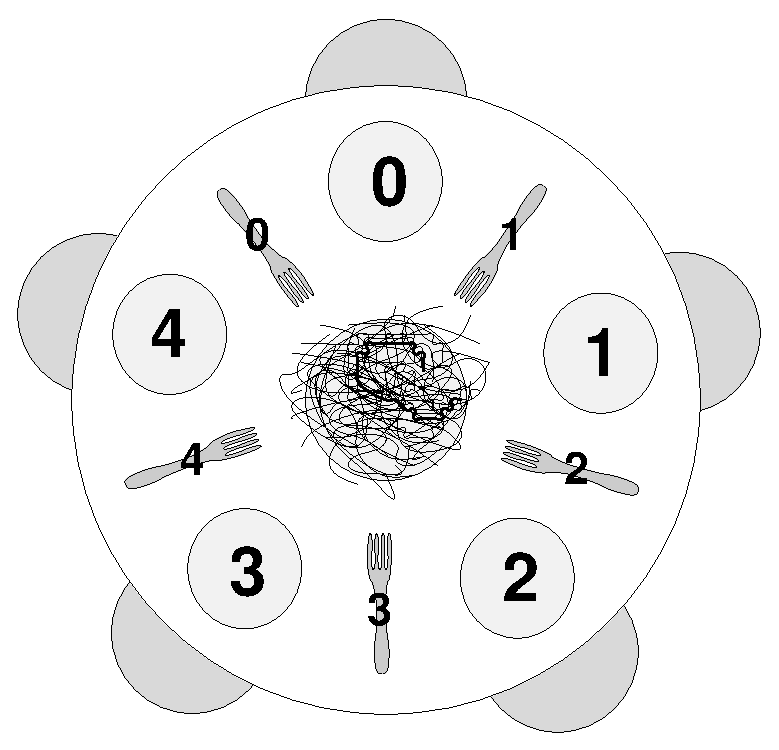
\includegraphics[height=2in]{table.eps}}

Assuming that the philosophers know how to {\tt think} and {\tt eat},
our job is to write a version of {\tt get\_forks} and {\tt put\_forks}
that satisfies the following constraints:

\begin{itemize}

\item Only one philosopher can hold a fork at a time.

\item It must be impossible for a deadlock to occur.

\item It must be impossible for a philosopher to starve waiting
for a fork.

\item It must be possible for more than one philosopher
to eat at the same time.

\end{itemize}

The last requirement is one way of saying that the solution
should be efficient; that is, it should allow the maximum amount
of concurrency.

We make no assumption about how long {\tt eat} and {\tt think} take,
except that {\tt eat} has to terminate eventually.  Otherwise, the
third constraint is impossible---if a philosopher keeps one of the
forks forever, nothing can prevent the neighbors from starving.

To make it easy for philosophers to refer to their forks,
we can use the functions {\tt left} and {\tt right}:

\begin{lstlisting}[title={Which fork?}]{}
def left(i): return i
def right(i): return (i + 1) % 5
\end{lstlisting}

The {\tt \%} operator wraps around when it gets to 5, so
{\tt (4 + 1) \% 5 = 0}.

Since we have to enforce exclusive access to the forks,
it is natural to use a list of Semaphores, one for
each fork.  Initially, all the forks are available.

\begin{lstlisting}[title={Variables for dining philosophers}]{}
forks = [Semaphore(1) for i in range(5)]
\end{lstlisting}

This notation for initializing a list might be unfamiliar to
readers who don't use Python.  The {\tt range} function returns
a list with 5 elements; for each element of this list, Python
creates a Semaphore with initial value 1 and assembles the
result in a list named {\tt forks}.

Here is an initial attempt at {\tt get\_fork} and {\tt put\_fork}:

\begin{lstlisting}[title={Dining philosophers non-solution}]{}
def get_forks(i):
    fork[right(i)].wait()
    fork[left(i)].wait()

def put_forks(i):
    fork[right(i)].signal()
    fork[left(i)].signal()
\end{lstlisting}

It's clear that this solution satisfies the first constraint, but
we can be pretty sure it doesn't satisfy the other two, because
if it did, this wouldn't be an interesting problem and you would
be reading Chapter~\ref{next}.

Puzzle: what's wrong?


\clearemptydoublepage
\subsection{Deadlock \#5}

The problem is that the table is round.  As a result, each philosopher
can pick up a fork and then wait forever for the other fork.  Deadlock!

Puzzle: write a solution to this problem that prevents deadlock.

Hint: one way to avoid deadlock is to think about the conditions
that make deadlock possible and then change one of those conditions.
In this case, the deadlock is fairly fragile---a very small change
breaks it.

\clearemptydoublepage
\subsection{Dining philosophers hint \#1}

If only four philosophers are allowed at the table at a time,
deadlock is impossible.

First, convince yourself that this claim is true, then write code that
limits the number of philosophers at the table.


\clearemptydoublepage
\subsection{Dining philosophers solution \#1}

If there are only four philosophers at the table, then in the
worst case each one picks up a fork.  Even then, there is a fork
left on the table, and that fork has two neighbors, each of
which is holding another fork.  Therefore, either of these
neighbors can pick up the remaining fork and eat.

We can control the number of philosophers at the table with
a Multiplex named {\tt footman} that is initialized to 4.
Then the solution looks like this:

\begin{lstlisting}[title={Dining philosophers solution \#1}]{}
def get_forks(i):
    footman.wait()
    fork[right(i)].wait()
    fork[left(i)].wait()

def put_forks(i):
    fork[right(i)].signal()
    fork[left(i)].signal()
    footman.signal()
\end{lstlisting}

In addition to avoiding deadlock, this solution also guarantees that
no philosopher starves.
Imagine that you
are sitting at the table and both of your neighbors are eating.  You
are blocked waiting for your right fork.  Eventually your right
neighbor will put it down, because {\tt eat} can't run forever.  Since
you are the only thread waiting for that fork, you will necessarily
get it next.  By a similar argument, you cannot starve waiting for
your left fork.

Therefore, the time a philosopher can spend at the table is bounded.
That implies that the wait time to get into the room is also bounded,
as long as {\tt footman} has Property 4 (see Section ~\ref{props}).

This solution shows that
by controlling the number of philosophers, we can avoid deadlock.
Another way to avoid deadlock is to change the order in which the
philosophers pick up forks.  In the original non-solution, the
philosophers are ``righties''; that is, they pick up the right fork
first.  But what happens if Philosopher 0 is a leftie?

Puzzle: prove that if there is at least one leftie and at least one
rightie, then deadlock is not possible.

Hint: deadlock can only occur when all 5 philosophers are holding
one fork and waiting, forever, for the other.  Otherwise, one of
them could get both forks, eat, and leave.

The proof works by contradiction.  First, assume that deadlock is
possible.  Then choose one of the supposedly deadlocked philosophers.
If she's a leftie, you can prove that the philosophers are all
lefties, which is a contradiction.  Similarly, if she's a rightie, you
can prove that they are all righties.  Either way you get a
contradiction; therefore, deadlock is not possible.


\clearemptydoublepage
\subsection{Dining philosopher's solution \#2}

In the asymmetric solution to the Dining philosophers problem,
there has to be at least one leftie and at least one rightie at
the table.  In that case, deadlock is impossible.  The previous
hint outlines the proof.  Here are the details.

Again, if deadlock is possible, it occurs when all 5 philosophers
are holding one fork and waiting for the other.  If we assume that
Philosopher $j$ is a leftie, then she must be holding her left
fork and waiting for her right.  Therefore her neighbor to the right,
Philosopher $k$, must be holding his left fork and waiting for
his right neighbor; in other words, Philosopher $k$ must be a leftie.
Repeating the same argument, we can prove that the philosophers
are all lefties, which contradicts the original claim that there
is at least one rightie.  Therefore deadlock is not possible.

The same argument we used for the previous solution also proves
that starvation is impossible for this solution.


\clearemptydoublepage
\subsection{Tanenbaum's solution}

There is nothing wrong with the previous solutions, but just for
completeness, let's look at some alternatives.  One of the best known
is the one that appears in Tanenbaum's popular operating systems
textbook \cite{tanenbaum}.
For each philosopher there is a state variable that
indicates whether the philosopher is thinking, eating, or waiting to
eat (``hungry'') and a semaphore that indicates whether the
philosopher can start eating.  Here are the variables:

\begin{lstlisting}[title={Variables for Tanenbaum's solution}]{}
state = ['thinking'] * 5
sem = [Semaphore(0) for i in range(5)]
mutex = Semaphore(1)
\end{lstlisting}

The initial value of {\tt state} is a list of 5 copies of {\tt
'thinking'}.  {\tt sem} is a list of 5 semaphores with the initial
value 0.  Here is the code:

\begin{lstlisting}[title={Tanenbaum's solution}]{}
def get_fork(i):
    mutex.wait()
    state[i] = 'hungry'
    test(i)
    mutex.signal()
    sem[i].wait()

def put_fork(i):
    mutex.wait()
    state[i] = 'thinking'
    test(right(i))
    test(left(i))
    mutex.signal()

def test(i):
    if state[i] == 'hungry' and
    state[left (i)]  != 'eating' and
    state[right (i)] != 'eating':
        state[i] = 'eating'
        sem[i].signal()
\end{lstlisting}

% NOTE: need to fix this; see email from David Furcy.

The {\tt test} function checks whether the $i$th philosopher can
start eating, which he can if he is hungry and
neither of his neighbors are eating.  If so, the {\tt test} signals
semaphore $i$.

There are two ways a philosopher gets to eat.  In the first case, the
philosopher executes {\tt get\_forks}, finds the forks available, and
proceeds immediately.  In the second case, one of the neighbors is
eating and the philosopher blocks on its own semaphore.  Eventually,
one of the neighbors will finish, at which point it executes {\tt
test} on both of its neighbors.  It is possible that both tests
will succeed, in which case the neighbors can run concurrently.
The order of the two tests doesn't matter.

In order to access {\tt state} or invoke {\tt test}, a thread
has to hold {\tt mutex}.  Thus, the operation of checking and
updating the array is atomic.  Since a philosopher can only proceed
when we know both forks are available, exclusive access to the forks
is guaranteed.

No deadlock is possible, because the only semaphore that is accessed
by more than one philosopher is {\tt mutex}, and no thread executes
{\tt wait} while holding {\tt mutex}.

But again, starvation is tricky.

Puzzle: Either convince yourself that Tanenbaum's solution prevents
starvation or find a repeating pattern that allows a thread to starve
while other threads make progress.


\clearemptydoublepage
\subsection{Starving Tanenbaums}

Unfortunately, this solution is not starvation-free.  Gingras
demonstrated that there are repeating patterns that allow a
thread to wait forever while other threads come and go
\cite{gingras90dining}.

Imagine that we are trying to starve Philosopher 0.  Initially,
2 and 4 are at the table and 1 and 3 are hungry.  Imagine that 2 gets up and
1 sit downs; then 4 gets up and 3 sits down.
Now we are in the mirror image of the starting position.

If 3 gets up and 4 sits
down, and then 1 gets up and 2 sits down, we are back
where we started.  We could repeat the cycle indefinitely and
Philosopher 0 would starve.

So, Tanenbaum's solution doesn't satisfy all the requirements.




\clearemptydoublepage
\section {Cigarette smokers problem}

The cigarette smokers problem was originally presented by
Suhas Patil \cite{patil}, who claimed that it cannot be solved with
semaphores.  That claim comes with some qualifications, but in
any case the problem is interesting and challenging.

Four threads are involved: an agent and three smokers.  The smokers
loop forever, first waiting for ingredients, then making and smoking
cigarettes.  The ingredients are tobacco, paper, and matches.

We assume that the agent has an infinite supply of all three
ingredients, and each smoker has an infinite supply of one of
the ingredients; that is, one smoker has matches, another has
paper, and the third has tobacco.

The agent repeatedly chooses two different ingredients at random
and makes them available to the smokers.  Depending on which
ingredients are chosen, the smoker with the complementary ingredient
should pick up both resources and proceed.

For example, if the agent puts out tobacco and paper, the
smoker with the matches should pick up both ingredients, make
a cigarette, and then signal the agent.

To explain the premise, the agent represents an operating system that
allocates resources, and the smokers represent applications that need
resources.  The problem is to make sure that if resources are
available that would allow one or more applications to proceed,
those applications should be woken up.  Conversely, we want to avoid
waking an application if it cannot proceed.



Based on this premise, there are three versions of this problem
that often appear in textbooks:

\begin{description}

\item[The impossible version:] Patil's version imposes restrictions on
the solution.  First, you are not allowed to modify the agent code.
If the agent represents an operating system, it makes sense to assume
that you don't want to modify it every time a new application comes
along.  The second restriction is that you can't use conditional
statements or an array of semaphores.  With these constraints, the
problem cannot be solved, but as Parnas points out, the second
restriction is pretty artificial \cite{Parnas}.  With constraints like
these, a lot of problems become unsolvable.

\item[The interesting version:] This version keeps the first
restriction---you can't change the agent code---but it drops the others.

\item[The trivial version:] In some textbooks, the problem specifies
that the agent should signal the smoker that should go next, according
to the ingredients that are available.  This version of the problem
is uninteresting because it makes the whole premise, the ingredients
and the cigarettes, irrelevant.  Also, as a practical matter, it is
probably not a good idea to require the agent to know about the other
threads and what they are waiting for.  Finally, this version of
the problem is just too easy.

\end{description}

Naturally, we will focus on the interesting version.  To complete
the statement of the problem, we need to specify the agent code.
The agent uses the following semaphores:

\begin{lstlisting}[title={Agent semaphores}]{}
agentSem = Semaphore(1)
tobacco = Semaphore(0)
paper = Semaphore(0)
match = Semaphore(0)
\end{lstlisting}

The agent is actually made up of three concurrent
threads, Agent A, Agent B and Agent C.  Each waits on
{\tt agentSem}; each time {\tt agentSem} is signaled,
one of the Agents wakes up and provides ingredients by
signaling two semaphores.

\begin{lstlisting}[title={Agent A code}]{}
agentSem.wait()
tobacco.signal()
paper.signal()
\end{lstlisting}

\begin{lstlisting}[title={Agent B code}]{}
agentSem.wait()
paper.signal()
match.signal()
\end{lstlisting}

\begin{lstlisting}[title={Agent C code}]{}
agentSem.wait()
tobacco.signal()
match.signal()
\end{lstlisting}

This problem is hard because the natural solution does not
work.  It is tempting to write something like:

\begin{lstlisting}[title={Smoker with matches}]{}
tobacco.wait()
paper.wait()
agentSem.signal()
\end{lstlisting}

\begin{lstlisting}[title={Smoker with tobacco}]{}
paper.wait()
match.wait()
agentSem.signal()
\end{lstlisting}

\begin{lstlisting}[title={Smoker with paper}]{}
tobacco.wait()
match.wait()
agentSem.signal()
\end{lstlisting}

What's wrong with this solution?

\clearemptydoublepage
\subsection{Deadlock \#6}

The problem with the previous solution is the possibility
of deadlock.  Imagine that the agent puts out tobacco and
paper.  Since the smoker with matches is waiting on {\tt tobacco},
it might be unblocked.  But the smoker with tobacco is
waiting on {\tt paper}, so it is possible (even likely) that
it will also be unblocked.  Then the first thread will block
on {\tt paper} and the second will block on {\tt match}.
Deadlock!

\clearemptydoublepage
\subsection{Smokers problem hint}

The solution proposed by Parnas uses three helper threads
called ``pushers'' that respond to the signals from the agent,
keep track of the available ingredients, and signal the
appropriate smoker.

The additional variables and semaphores are

\begin{lstlisting}[title={Smokers problem hint}]{}
isTobacco = isPaper = isMatch = False
tobaccoSem = Semaphore(0)
paperSem = Semaphore(0)
matchSem = Semaphore(0)
\end{lstlisting}

The boolean variables indicate whether or not an ingredient
is on the table.  The pushers use {\tt tobaccoSem} to signal
the smoker with tobacco, and the other semaphores likewise.


\clearemptydoublepage
\subsection{Smoker problem solution}

Here is the code for one of the pushers:

\begin{lstlisting}[title={Pusher A}]{}
tobacco.wait()
mutex.wait()
    if isPaper:
        isPaper = False
        matchSem.signal()
    elif isMatch:
        isMatch = False
        paperSem.signal()
    else: 
        isTobacco = True
mutex.signal()
\end{lstlisting}

This pusher wakes up any time there is tobacco on the
table.  If it finds {\tt isPaper} true, it knows that
Pusher B has already run, so it can signal the smoker
with matches.  Similarly, if it finds a match on the
table, it can signal the smoker with paper.

But if Pusher A runs first, then it will find both
{\tt isPaper} and {\tt isMatch} false.  It cannot signal
any of the smokers, so it sets {\tt isTobacco}.

The other pushers are similar.  Since the pushers do all
the real work, the smoker code is trivial:

\begin{lstlisting}[title={Smoker with tobacco}]{}
tobaccoSem.wait()
makeCigarette()
agentSem.signal()
smoke()
\end{lstlisting}

Parnas presents a similar solution that assembles the
boolean variables, bitwise, into an integer, and then
uses the integer as an index into an array of semaphores.
That way he can avoid using conditionals (one of the
artificial constraints).  The resulting code is a bit
more concise, but its function is not as obvious.


\subsection{Generalized Smokers Problem}

Parnas suggested that the smokers problem becomes more
difficult if we modify the agent, eliminating the requirement
that the agent wait after putting out ingredients.  In this
case, there might be multiple instances of an ingredient on
the table.

Puzzle: modify the previous solution to deal with this
variation.

\clearemptydoublepage
\subsection{Generalized Smokers Problem Hint}

If the agents don't wait for the smokers, ingredients might
accumulate on the table.  Instead of using boolean values to
keep track of ingredients, we need integers to count them.

\begin{lstlisting}[title={Generalized Smokers problem hint}]{}
numTobacco = numPaper = numMatch = 0
\end{lstlisting}


\clearemptydoublepage
\subsection{Generalized Smokers Problem Solution}
\label{smoker}

Here is the modified code for Pusher A:

\begin{lstlisting}[title={Pusher A}]{}
tobacco.wait()
mutex.wait()
    if numPaper:
        numPaper -= 1
        matchSem.signal()
    elif numMatch:
        numMatch -= 1
        paperSem.signal()
    else: 
        numTobacco += 1
mutex.signal()
\end{lstlisting}

One way to visualize this problem is to imagine that when an
Agent runs, it creates two pushers, gives each of them one ingredient,
and puts them in a room with all the other pushers.  Because of the
mutex, the pushers file into a room where there are
three sleeping smokers and a table.  One at a time, each pusher enters
the room and checks the ingredients on the table.  If he can
assemble a complete set of ingredients, he takes them off the table
and wakes the corresponding smoker.  If not, he leaves his ingredient
on the table and leaves without waking anyone.

This is an example of a pattern we will see several times, which
I call a {\bf scoreboard}.  The variables {\tt numPaper}, {\tt numTobacco}
and {\tt numMatch} keep track of the state of the system.  As each
thread files through the mutex, it checks the state as if looking
at the scoreboard, and reacts accordingly.


\clearemptydoublepage
